\documentclass[journal=jacsat,manuscript=article]{achemso}
\SectionNumbersOn
\usepackage[version=3]{mhchem}
\usepackage{xcolor}
\usepackage{amsmath,amssymb}
\usepackage{graphicx}
\usepackage{booktabs}
\usepackage{subcaption}
\newcommand*\mycommand[1]{\texttt{\emph{#1}}}
\author{Eric Boittier}
\author{Mike Devereux}
\author{Markus Meuwly}
\email{m.meuwly@unibas.ch}
\phone{+41 (0)61 2073821}
\affiliation[University of Basel]
{Department of Chemistry, University of Basel, Switzerland}

\title[ Energy Decomposition Analysis ] { SI: Energy Decomposition Analysis }


\begin{document}

\begin{abstract}
 This report summaries the findings from 
ab initio WFT and energy decomposition analysis. These results were used to fit
classical force fields intended for the simulation. The agreement between 
the ab initio data and the data modelled by molecular mechanics force fields is analyzed.

\end{abstract}

\clearpage
\begin{table}[b!]
\centering
\caption{Summary statistics for the energy data.}
\label{tab:energy_stats}
\begin{tabular}{lrrrr}
\toprule
{} &  M\_ENERGY &  C\_ENERGY &  P\_intE &    intE \\
\midrule
count &    500.00 &    500.00 &  500.00 &  500.00 \\
mean  &  -1527.15 &  -1527.24 &  -57.98 &  -60.22 \\
std   &      0.01 &      0.02 &   10.63 &   13.22 \\
min   &  -1527.17 &  -1527.33 &  -91.34 & -102.62 \\
25\%   &  -1527.15 &  -1527.26 &  -65.72 &  -68.75 \\
50\%   &  -1527.15 &  -1527.24 &  -58.34 &  -60.85 \\
75\%   &  -1527.14 &  -1527.23 &  -50.43 &  -51.07 \\
max   &  -1527.12 &  -1527.18 &  -27.18 &  -25.02 \\
\bottomrule
\end{tabular}
\end{table}

\begin{table}[b!]
\centering
\caption{Summary statistics for the energy data.}
\label{tab:energy_stats}
\begin{tabular}{lrrrr}
\toprule
{} &  M\_ENERGY &  C\_ENERGY &  P\_intE &   intE \\
\midrule
count &    201.00 &    201.00 &  201.00 & 201.00 \\
mean  & -19187.35 & -19187.37 &  -13.20 & -12.90 \\
std   &      0.01 &      0.01 &    4.24 &   4.16 \\
min   & -19187.37 & -19187.40 &  -25.26 & -24.25 \\
25\%   & -19187.36 & -19187.38 &  -16.11 & -15.95 \\
50\%   & -19187.35 & -19187.37 &  -13.24 & -12.83 \\
75\%   & -19187.34 & -19187.36 &  -10.35 & -10.04 \\
max   & -19187.31 & -19187.32 &   -2.91 &  -2.59 \\
\bottomrule
\end{tabular}
\end{table}

\subsection{waterclusterpbe0dzpc}
\subsubsection{Distribution of Energies} 
 The following figures show the distribution of energies for the monomers, pairs, and clusters.

\begin{figure}
    \centering
    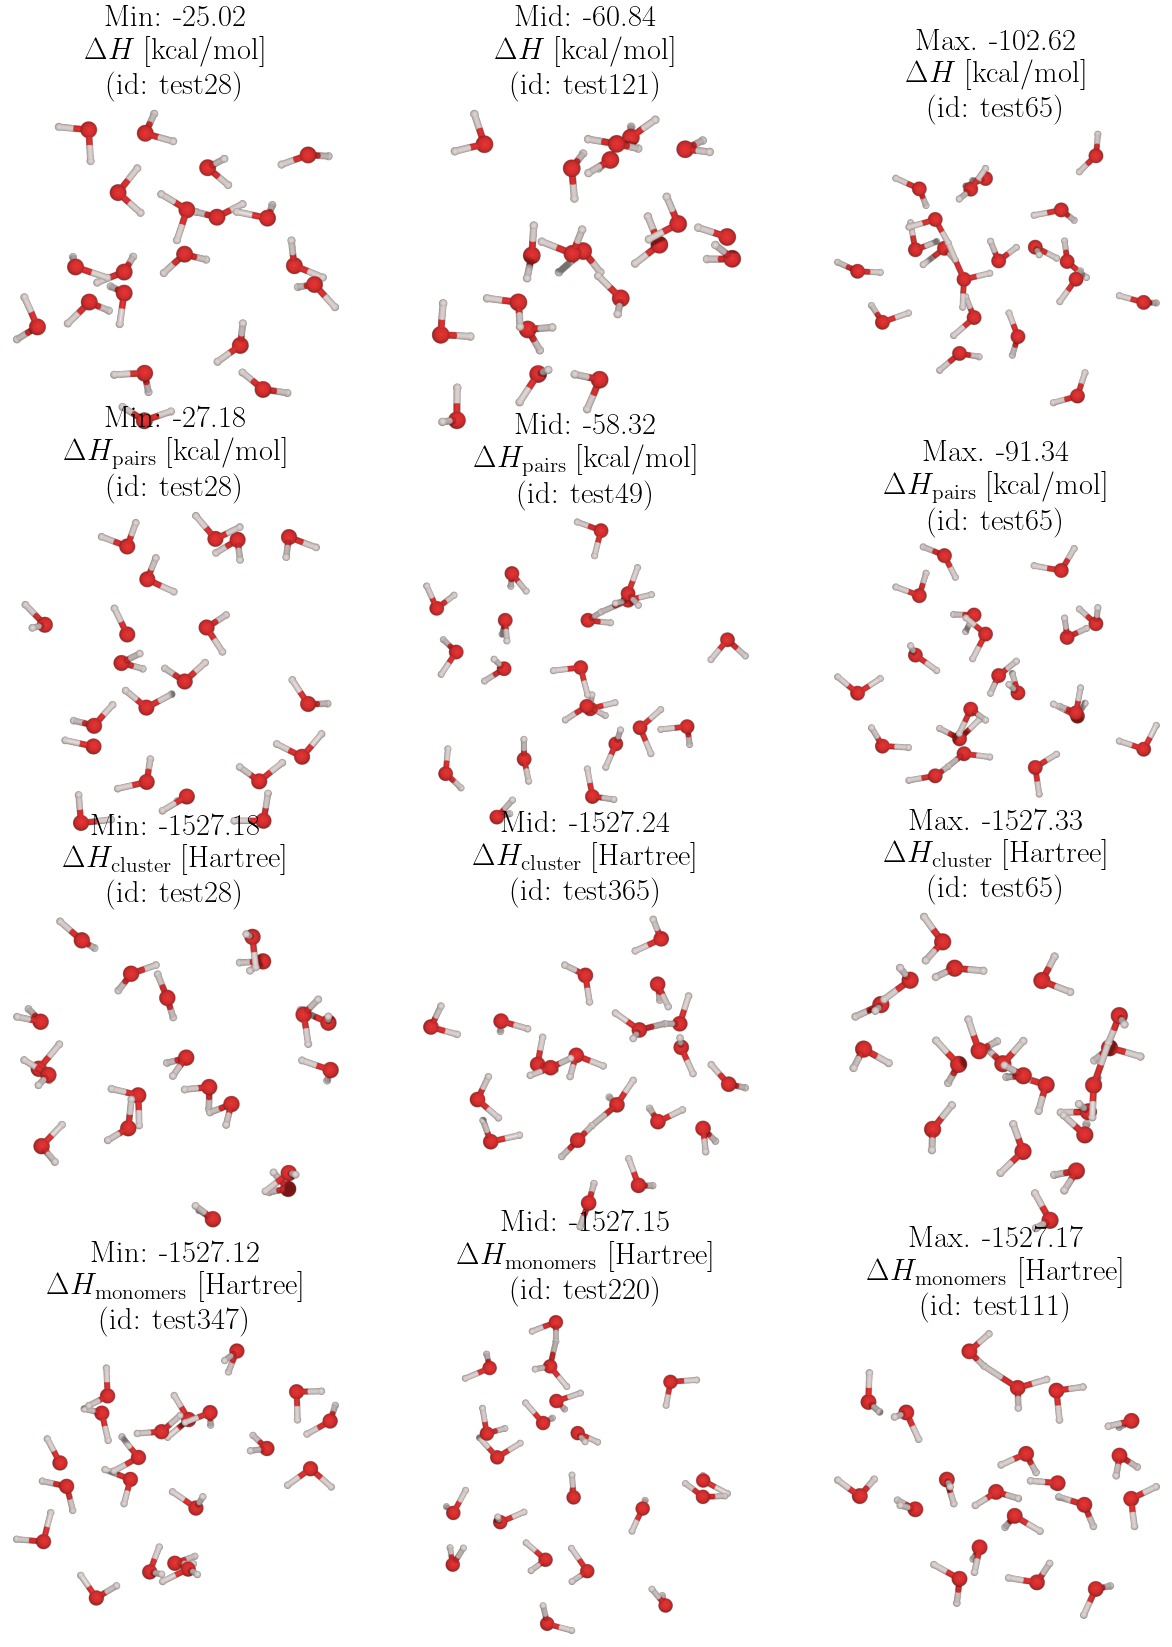
\includegraphics[width=0.85\textwidth]{figures/Waterclustersmols}
    \caption{ Waterclusters }
    \label{fig:Waterclustersmols}
\end{figure}

\begin{figure}
    \centering
    \includegraphics[width=0.5\textwidth]{figures/MENERGY}
    \caption{ Distribution of  M E N E R G Y }
    \label{fig:singlekey}
\end{figure}

\begin{figure}
    \centering
    \includegraphics[width=1.0\textwidth]{figures/intE_P_intE}
    \caption{ Analysis of $\Delta H$ [kcal/mol] and $\Delta H{\mathrm{pairs}}$ [kcal/mol] }
    \label{fig:_intE_P_intE}
\end{figure}

\begin{figure}
    \centering
    \includegraphics[width=1.0\textwidth]{figures/C_ENERGY_M_ENERGY}
    \caption{ Analysis of $\Delta H{\mathrm{cluster}}$ [Hartree] and $\Delta H{\mathrm{monomers}}$ [Hartree] }
    \label{fig:_C_ENERGY_M_ENERGY}
\end{figure}
\newpage 
 \subsection{Fitting Results}
\subsection{dcmpbe0dzpc}
\subsubsection{Distribution of Energies} 
 The following figures show the distribution of energies for the monomers, pairs, and clusters.

\begin{figure}
    \centering
    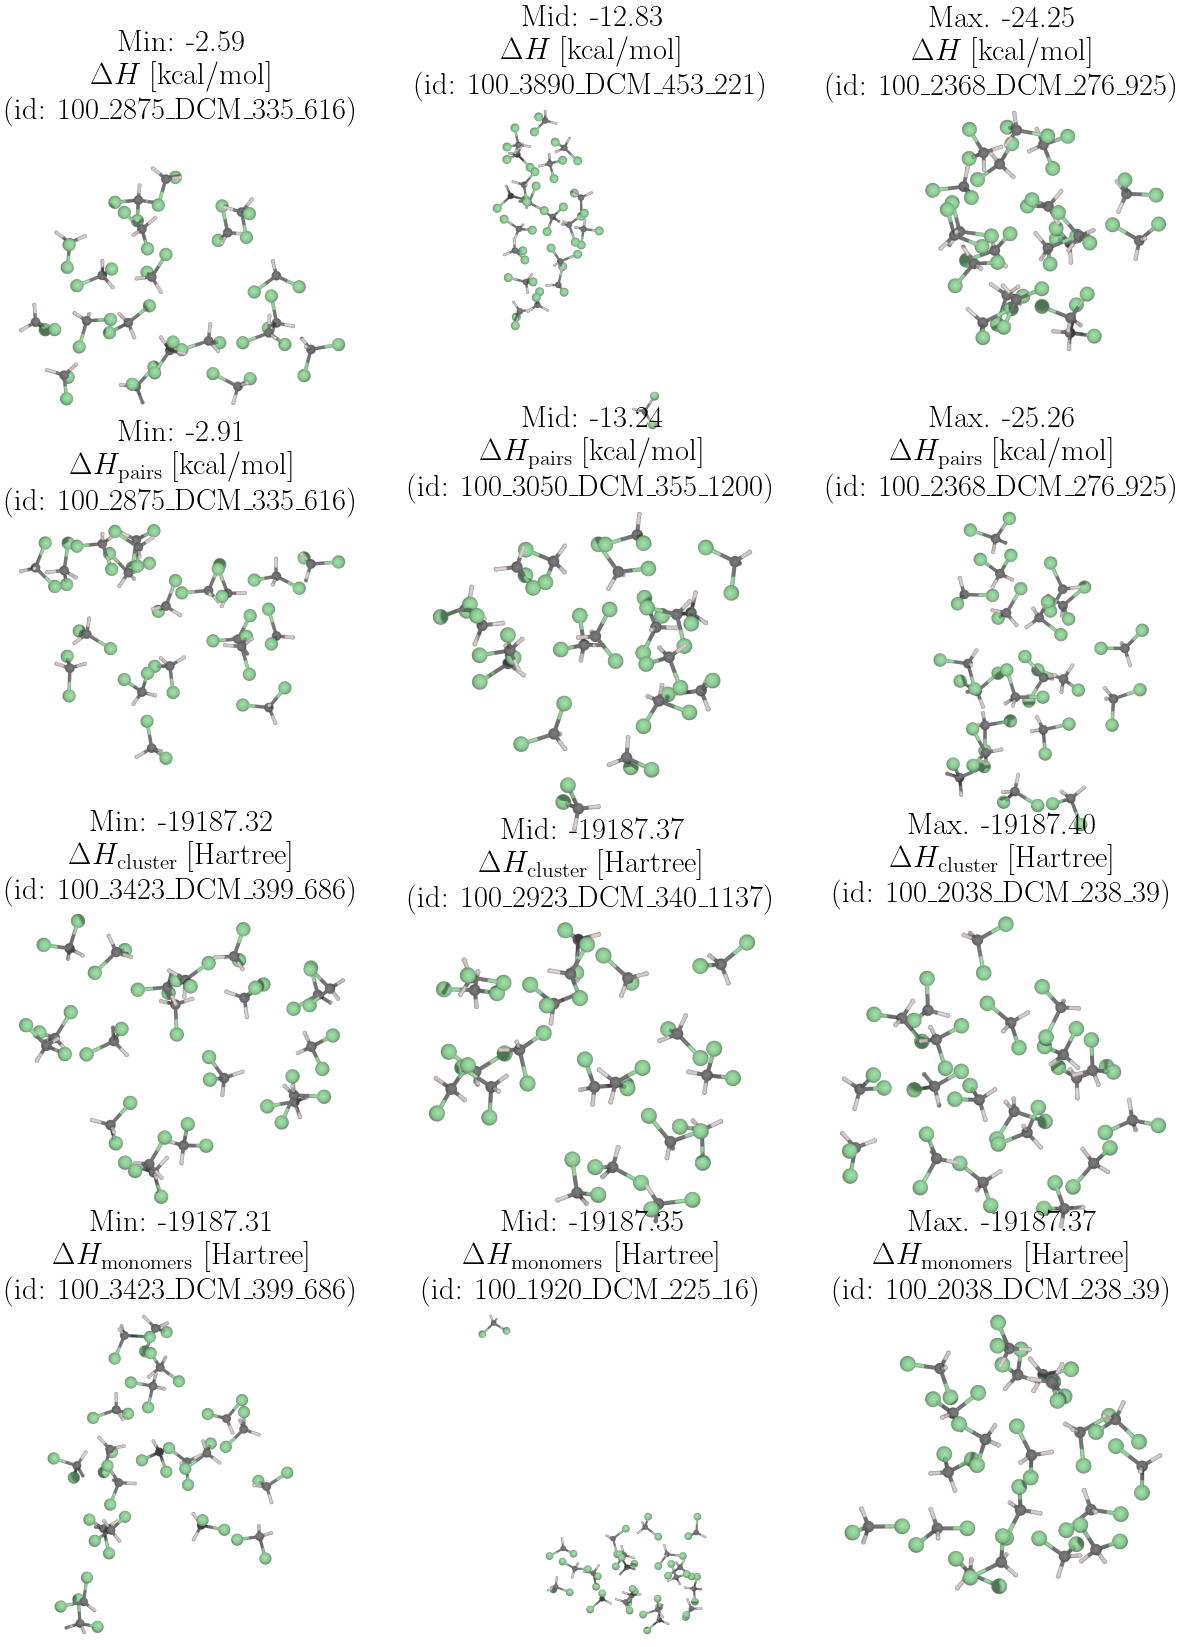
\includegraphics[width=0.85\textwidth]{figures/DCMclustersmols}
    \caption{ DCMclusters }
    \label{fig:DCMclustersmols}
\end{figure}

\begin{figure}
    \centering
    \includegraphics[width=0.5\textwidth]{figures/MENERGY}
    \caption{ Distribution of  M E N E R G Y }
    \label{fig:singlekey}
\end{figure}

\begin{figure}
    \centering
    \includegraphics[width=1.0\textwidth]{figures/intE_P_intE}
    \caption{ Analysis of $\Delta H$ [kcal/mol] and $\Delta H{\mathrm{pairs}}$ [kcal/mol] }
    \label{fig:_intE_P_intE}
\end{figure}

\begin{figure}
    \centering
    \includegraphics[width=1.0\textwidth]{figures/C_ENERGY_M_ENERGY}
    \caption{ Analysis of $\Delta H{\mathrm{cluster}}$ [Hartree] and $\Delta H{\mathrm{monomers}}$ [Hartree] }
    \label{fig:_C_ENERGY_M_ENERGY}
\end{figure}
\newpage 
 \subsection{Fitting Results}

\end{document}